%=======================================================================
% Federated GRU Intrusion Detection with an Ascon-Sealed Bidirectional
% Weight Channel for Smart-Agriculture IoT
%
% Compiles on Overleaf as-is: IEEEtran is preinstalled there.
%   Compiler: pdfLaTeX    Bibliography: BibTeX
%
% Figures live in paper/figures/. Any figure not yet generated renders as a
% labelled placeholder box via \figbox, so the document always compiles.
%
% STATUS MARKERS used in this draft:
%   \todo{...}     work still owed
%   \verifycite{}  citation whose record or attributed claim is unconfirmed
%=======================================================================
\documentclass[conference]{IEEEtran}
\IEEEoverridecommandlockouts

\usepackage{cite}
\usepackage{amsmath,amssymb,amsfonts}
\usepackage{algorithm}
\usepackage{algpseudocode}
\usepackage{graphicx}
\usepackage{booktabs}
\usepackage{multirow}
\usepackage{xcolor}
\usepackage{url}
\usepackage[hidelinks]{hyperref}
\graphicspath{{figures/}{diagrams/}}

% --- draft aids -------------------------------------------------------
\newcommand{\todo}[1]{\textcolor{red}{\textbf{[TODO: #1]}}}
\newcommand{\verifycite}[1]{\textcolor{orange}{$^{\mathrm{[verify]}}$}}
% Placeholder so the paper compiles before a figure exists.
\newcommand{\figbox}[2]{%
  \fbox{\begin{minipage}[c][#1][c]{0.94\linewidth}\centering
    \textcolor{gray}{\small FIGURE PENDING\\[2pt]#2}
  \end{minipage}}}

\begin{document}

\title{Federated GRU Intrusion Detection with an Ascon-Sealed\\
Bidirectional Weight Channel for Smart-Agriculture IoT}

\author{%
\IEEEauthorblockN{Abhishek Jadli}
\IEEEauthorblockA{\textit{Department of Computer Science}\\
\textit{Vellore Institute of Technology}\\
Chennai, India\\
abhishek.jadli2023@vitstudent.ac.in}
\and
\IEEEauthorblockN{Aryan Agarwal}
\IEEEauthorblockA{\textit{Department of Computer Science}\\
\textit{Vellore Institute of Technology}\\
Chennai, India\\
aryan.agarwal2023@vitstudent.ac.in}
\and
\IEEEauthorblockN{Advait Amit Malviya}
\IEEEauthorblockA{\textit{Department of Computer Science}\\
\textit{Vellore Institute of Technology}\\
Chennai, India\\
advaitamit.malviya2023@vitstudent.ac.in}
\and
\IEEEauthorblockN{Vijayprabhakaran K}
\IEEEauthorblockA{\textit{School of Computer Science and Engineering}\\
\textit{Vellore Institute of Technology}\\
Chennai, India}
}

\maketitle

%=======================================================================
\begin{abstract}
Federated learning is the standard answer to training an intrusion detector across sites
that cannot pool their traffic, but the parameters it exchanges are themselves carried over
the untrusted network the detector exists to protect, and the literature that studies those
exchanges rarely says what the detector's verdict should then do to the data path. We present
a smart-agriculture intrusion detection system in which a gated recurrent detector runs on each
farm's edge gateway, every parameter vector crossing between a local detector and the
aggregator is sealed with Ascon-AEAD128 in both directions under per-client per-direction keys,
and the verdict selects between two structurally disjoint data paths: benign readings leave over
TLS, malicious readings never leave at all.
%
On CICIoT2023 the centralised detector reaches macro-F1 $0.8297 \pm 0.0013$, and recurrence
accounts for $+0.2322$ of that against an identical-budget multilayer perceptron. Federating
three farms recovers 82.4\% of the gap between local-only training and pooling, and
\emph{every} farm scores better federated than alone---$+0.1338$, $+0.0789$ and $+0.0516$
macro-F1---including one whose partition was missing attack classes entirely, which rises from
$0.6145$ to $0.8145$.
%
A 21-point sweep over client counts $K \in \{3,\dots,50\}$ shows the architecture degrades
gracefully in aggregate ($-0.079$ macro-F1 at $K=50$) while the rarest class falls $0.642
\rightarrow 0.386$, a 40\% relative collapse that macro-F1 alone conceals.
%
We validate the complete topology software-in-the-loop before any hardware: ten containerised
processes at the target CPU architecture completed 20 federated rounds with 120 sealed frames
and zero rejections, and the disjointness property held across 4{,}239 malicious readings with
none reaching the cloud, cross-checked against the receiver's own independent count.
%
We report two negative results. Zero-shot transfer to an unseen corpus collapses, replicating a
documented field-wide failure; and we show that a safety property can pass vacuously---an earlier
run of ours satisfied the disjointness assertion on a single malicious reading, which a
10\%-leaking system would also have passed nine times in ten.
\end{abstract}

\begin{IEEEkeywords}
intrusion detection, federated learning, Ascon, authenticated encryption, lightweight
cryptography, smart agriculture, Internet of Things, gated recurrent unit
\end{IEEEkeywords}

%=======================================================================
\section{Introduction}
\todo{write. Frame from the deployment: a farm gateway sees its own traffic only; pooling is
refused; the parameter exchange is the new exposure; and the verdict has to govern the data path.}

\subsection{Contributions}
This paper is an empirical study of a built and measured system. Its contributions are:

\begin{enumerate}
  \item \textbf{An Ascon-sealed bidirectional weight channel.} Every client update and every
  global-state download is an AEAD frame under a per-client, per-direction key, with associated
  data binding the client identity, round index, direction and schema version
  (Eq.~\eqref{eq:weightad}). The aggregator never applies a frame that opens to $\bot$. We
  report 120 sealed frames across 20 rounds with zero rejections and a measured
  271{,}883 bytes per client per round.
  \item \textbf{A per-client measurement of what federating is worth}, rather than a global
  average: every farm improves, and a farm whose partition lacked attack classes still gains
  $0.2000$ macro-F1 from the others' parameters.
  \item \textbf{A client-count study} over 21 configurations that separates aggregate
  degradation from rare-class collapse, and locates the onset of the second descent at the
  pigeonhole bound implied by the rarest class's block count (Eq.~\eqref{eq:pigeonhole}).
  \item \textbf{Dataset selection decided by measurement.} Three corpora were characterised and
  trained on; two were rejected, and the measurements that rejected them are reported rather
  than the choice merely asserted.
  \item \textbf{Software-in-the-loop validation of the full topology} before hardware exists,
  including the configuration errors that made two earlier runs invalid.
  \item \textbf{Two negative results}, one replicating a field-wide generalisation failure and
  one methodological: a safety property reported as satisfied carries no information unless the
  number of opportunities to violate it is reported with it.
\end{enumerate}

%=======================================================================
\section{Background and Related Work}

\subsection{Ascon and Ascon-AEAD128}\label{sec:ascon}
Ascon is a family of lightweight authenticated-encryption and hashing algorithms designed by
Dobraunig, Eichlseder, Mendel and Schl\"affer~\cite{dobraunig2021ascon}. It is built from a
single 320-bit permutation applied in a sponge-based duplex mode: the state is initialised from
the key, nonce and an algorithm-specific initial value, associated data is absorbed, plaintext
is absorbed and ciphertext squeezed block by block, and a tag is extracted at finalisation. The
same permutation serves every stage, which is what makes the primitive small enough for a
constrained device and simple enough to mask against side channels. Ascon-128 and Ascon-128a
were selected as the primary choice for lightweight authenticated encryption in the final CAESAR
portfolio\verifycite{}.

In August 2025 NIST published SP~800-232~\cite{nist2025sp800232}, standardising
\textbf{Ascon-AEAD128} together with Ascon-Hash256, Ascon-XOF128 and Ascon-CXOF128. This system
uses Ascon-AEAD128 exclusively: a 128-bit key, a 128-bit nonce and a 128-bit tag.

One implementation detail is worth stating because it is a trap. \emph{The standardised
Ascon-AEAD128 is not the pre-standard Ascon-128 or Ascon-128a}: the initial values and the byte
order differ. A widely installed Python package named \texttt{ascon} implements only the
pre-standard variants, and a system built on it would interoperate with nothing that follows the
standard while passing its own round-trip tests. We therefore bind the designers' own C reference
implementation~\cite{asconc} and gate all cryptographic integration behind conformance to the
standard's known-answer vectors, which is asserted by a test that must pass before any other
cryptographic code is exercised. No primitive is implemented from scratch in this work.

\subsection{What Ascon protects here, and what it does not}
Ascon protects \emph{the model parameters}, in both directions, between each local detector and
the aggregator. It does not protect the telemetry on its way to the cloud; that hop uses TLS.
The reasoning is one cipher per hop with a stated threat for each: the parameter exchange
traverses the untrusted field network and is the channel this work introduces, whereas the
gateway-to-cloud hop is an ordinary authenticated transport problem already solved by TLS.
\todo{state the threat model formally in Section~\ref{sec:threat}}

\subsection{Review protocol}\label{sec:protocol}
A reading list assembled by judgement cannot be audited, so every candidate was scored against
six parameters, each on $\{0,1,2\}$ for a maximum of twelve. Sources were IEEE Xplore, the ACM
Digital Library, SpringerLink, MDPI, ScienceDirect, arXiv, the NIST Computer Security Resource
Center and Google Patents. Search strings combined four term groups: (\texttt{"federated
learning"} OR \texttt{FedAvg}), (\texttt{"intrusion detection"} OR \texttt{IDS} OR
\texttt{"anomaly detection"}), (\texttt{IoT} OR \texttt{IIoT} OR \texttt{"smart agriculture"} OR
\texttt{"precision agriculture"}), and (\texttt{Ascon} OR \texttt{"lightweight cryptography"} OR
\texttt{AEAD} OR \texttt{MQTT}).

\begin{table}[t]
\caption{Selection parameters. Each scored 0--2; admission at $s \ge 8$ of 12, with a zero on
P1 or P2 disqualifying regardless of total.}
\label{tab:params}
\centering\footnotesize
\begin{tabular}{@{}p{0.9cm}p{6.4cm}@{}}
\toprule
\textbf{} & \textbf{Scored on}\\
\midrule
P1 & Domain proximity: IoT, IIoT or agricultural network security rather than enterprise or vehicular\\
P2 & Method overlap: federated optimisation, recurrent sequence models, or lightweight AEAD\\
P3 & Benchmark comparability: CICIoT2023 or a comparable public IoT flow dataset\\
P4 & Evidential strength: peer-reviewed venue, stated protocol, metrics beyond accuracy\\
P5 & Recency: 2021 onward, with foundational exceptions where the method is still the reference\\
P6 & Gap-analytic value: states or exhibits a limitation this project can act on\\
\bottomrule
\end{tabular}
\end{table}

The threshold was set at eight so that a study had to be strong on \emph{both} domain proximity
and method overlap rather than compensating for weakness in one with strength in the other.
Applying the protocol yielded twenty studies, S1--S20, summarised in Table~\ref{tab:corpus}. Two
admissions need explaining. S2 and S3 fall outside the recency window and were admitted under the
foundational exception, federated averaging and its proximal variant still being the algorithms
against which later methods are measured. S13 was admitted \emph{because} it cuts against our own
architectural choice: it reports a tree ensemble outperforming the recurrent models it tested,
which is why Section~\ref{sec:fedresults} carries a random-forest baseline.

\begin{table*}[t]
\caption{Reviewed corpus (S1--S20), admitted under the protocol of Section~\ref{sec:protocol}.
FL: federated learning. AEAD: authenticated encryption with associated data. ``Relevance''
states what the study contributes to the present design or to the gap analysis.}
\label{tab:corpus}
\centering\footnotesize
\begin{tabular}{@{}llllp{6.3cm}@{}}
\toprule
 & \textbf{Focus} & \textbf{Method} & \textbf{Data / platform} & \textbf{Relevance to this work}\\
\midrule
S1~\cite{neto2023ciciot} & IoT attack benchmark & Testbed capture, 105 devices & CICIoT2023 & Supplies the corpus; establishes the imbalance and the packet-window record semantics\\
S2~\cite{mcmahan2017fedavg} & Decentralised training & FedAvg & Image benchmarks & Aggregation rule adopted, Eq.~\eqref{eq:fedavg}\\
S3~\cite{li2020fedprox} & Heterogeneous federation & FedProx & Mixed & Explains client drift under non-IID data; documented fallback if FedAvg diverges\\
S4~\cite{nguyen2021flsurvey} & FL for IoT & Survey & --- & Frames the bandwidth and governance motivation for federation\\
S5~\cite{hernandezramos2025fedidsreview} & Federated IDS & Systematic review & --- & Umbrella reference; source of the Thread~B limitations\\
S6~\cite{belarbi2023federated} & IoT IDS & Federated deep learning & IoT flow data & Confirms feasibility of federated deep detectors at the edge\\
S7~\cite{ruzafa2021ppfl} & Industrial IoT IDS & Privacy-preserving FL & Industrial data & Quantifies the privacy--utility trade-off we place out of scope\\
S8~\cite{karunamurthy2025optimal} & IoT IDS & Optimised FL & IoT benchmarks & Reports GRU clients sharing parameters to a central aggregator\\
S9~\cite{abdelaziz2025tabtransformer} & IoT IDS & FL + TabTransformer & N-BaIoT, UNSW-NB15, CICIoT2023 & Alternative architecture on the same benchmark\\
S10~\cite{okey2024cnngru} & IoT IDS & FL, CNN-GRU / LSTM-GRU, wFedAvg, wFedProx & CICIoT2023, FLNET2023 & \textbf{Closest prior work}; validates GRU + weighted FedAvg on our corpus at 98.25\% accuracy; stops at the label\\
S11~\cite{khraisat2025discoveriot} & IoT IDS & Privacy-preserving FL & IoT data & Evidence on privacy-preserving aggregation strategy\\
S12~\cite{distributediot2025dp} & Distributed IoT security & Adaptive weighting + per-device DP & Tabular IoT, Edge-IIoTset & Shows differential-privacy cost is modest; supports our future-work path\\
S13~\cite{bai2025ietinfsec} & IoT IDS & Nine ML/DL models; three aggregation rules & UNSW-NB15 & \textbf{Dissenting evidence}: a tree ensemble beat GRU/LSTM; motivates our random-forest baseline\\
S14~\cite{dobraunig2021ascon} & Lightweight AEAD & Ascon v1.2 design & --- & Primitive specification and design rationale\\
S15~\cite{khan2024asconasic} & Ascon hardware & ASIC realisation & Constrained hardware & Evidence of suitability for field-node cost budgets\\
S16~\cite{khan2022asconperf} & Ascon performance & Benchmarking & AI-enabled IoT devices & Latency and resource evidence on IoT-class hardware\\
S17~\cite{suleiman2026lweiot} & Lightweight encryption over IoT protocols & Ascon, PRESENT, SIMON, SPECK, ChaCha20 & MQTT and CoAP, ESP32 & Directly comparable protocol-level measurement methodology\\
S18~\cite{elhajj2024asconindustry40} & Industry 4.0 security & Ascon AEAD vs.\ AES-GCM & MQTT, digital twin & Memory and execution-time figures used in our constrained-device argument\\
S19~\cite{ozturk2025chaosascon} & IoRT data security & \emph{Chaos-based} Ascon variant & MQTT, Raspberry Pi 3B & Evidence Ascon-class cryptography runs on gateway hardware; \emph{not} evidence about the standardised variant\\
S20~\cite{fathy2023irrigation} & Precision agriculture & Lightweight cipher for irrigation & Agricultural IoT & Establishes the agricultural threat scenario for the telemetry channel; no detection layer\\
\bottomrule
\end{tabular}
\end{table*}

\subsection{Thread A: benchmark data and sequence-based detection}
CICIoT2023~\cite{neto2023ciciot} is the corpus this work trains on. It was built on a testbed of
105 real IoT devices and contains roughly 46.7~million labelled records with 46--47 flow-derived
features, spanning one benign class and 33 attack classes grouped into families. Two of its
properties drive the design.

Each record summarises a fixed-size \emph{packet window} rather than a single packet. The data is
therefore already aggregated once over time, and a recurrent model reading a sequence of records
performs a second-order temporal analysis: it observes how flow statistics evolve. That is the
justification for recurrence here, and it rests on the record semantics rather than on the
general observation that network traffic is sequential.

The class distribution is severely imbalanced, with a reported imbalance ratio near $5751$,
so a classifier predicting the majority class alone attains high accuracy while detecting nothing
of interest. Any evaluation on this corpus reporting accuracy alone is uninformative, which is
why macro-F1 and false-positive rate are treated as primary throughout.

Recurrent and convolutional-recurrent architectures dominate the applied
literature~\cite{okey2024cnngru,bai2025ietinfsec}. S13~\cite{bai2025ietinfsec} is the useful
dissent: benchmarking nine methods, it found a random forest strongest on tabular flow features,
then compared simple, weighted and difference-based aggregation rules federated over that model.

\textbf{Limitation across Thread A.} Papers building sequences from flow records frequently
shuffle rows before windowing, or do not state the ordering procedure at all. Where the source
data carries no timestamp or flow identifier, a sliding window is a \emph{positional} construct
and not a temporal one. We found this distinction rarely acknowledged; it is the
sequence-construction gap of Section~\ref{sec:gaps}.

\subsection{Thread B: federated learning for IoT intrusion detection}
Federated averaging~\cite{mcmahan2017fedavg} is the reference algorithm: clients perform local
stochastic gradient descent and the server averages parameters weighted by local sample count.
FedProx~\cite{li2020fedprox} adds a proximal term constraining client drift under statistical
heterogeneity, and is the standard citation for why non-identically distributed client data
degrades plain FedAvg. Broader context comes from a survey of federated learning for
IoT~\cite{nguyen2021flsurvey} and a systematic review of federated intrusion
detection~\cite{hernandezramos2025fedidsreview}.

Applied results are consistent in direction. Federated deep detectors reach accuracy close to
their centralised counterparts on IoT
benchmarks~\cite{belarbi2023federated,karunamurthy2025optimal}, including on CICIoT2023 itself.
Work on the industrial IoT quantifies the privacy--utility trade-off when differential privacy is
added~\cite{ruzafa2021ppfl}, and further studies report that tightening the privacy budget costs
only low single-digit percentage points of accuracy~\cite{distributediot2025dp}. Alternative
architectures~\cite{abdelaziz2025tabtransformer} and privacy-preserving
strategies~\cite{khraisat2025discoveriot} fill out the space.

S10~\cite{okey2024cnngru} is the closest prior work to our detection layer. It builds a federated
ensemble over CNN, GRU and LSTM with two aggregation functions, weighted FedAvg and weighted
FedProx, evaluated on CICIoT2023 and FLNET2023; CNN-GRU reaches 98.25\% accuracy on CICIoT2023 and
LSTM-GRU 93.36\% and 95.66\% on the two corpora respectively. It establishes that GRU plus
weighted federated averaging on CICIoT2023 is workable, which de-risks our detection design. It
does not consider what happens to traffic after classification, does not model a runtime IoT
stream, and is not set in an agricultural context.

\textbf{Limitations across Thread B.} Four recur, and they become four of the gaps in
Section~\ref{sec:gaps}. Privacy is asserted rather than bounded, many papers treating ``raw data
does not move'' as equivalent to privacy, which parameter-inversion attacks show it is not.
Client partitioning is under-specified, and a uniform random split is often described as
heterogeneous when it is identically distributed by construction. The local-only baseline is
usually absent, although it is the comparison that matters operationally, since local-only is what
an operator gets by declining to federate. And the pipeline terminates at a label.

\subsection{Thread C: lightweight authenticated encryption in deployment}
Performance evidence for Ascon on constrained platforms is substantial. An ASIC
realisation~\cite{khan2024asconasic} and benchmarking on AI-enabled IoT
devices~\cite{khan2022asconperf} establish suitability for field-node cost budgets. There are
also direct evaluations over IoT application protocols. LWE-IoT~\cite{suleiman2026lweiot} compares
Ascon, PRESENT, SIMON, SPECK and ChaCha20 over both MQTT and CoAP on ESP32 nodes across payload
sizes, which is the protocol-level measurement methodology closest to our own.

El-Hajj and Gebremariam~\cite{elhajj2024asconindustry40} validate Ascon against AES-GCM over MQTT
in an Industry~4.0 digital-twin setting, reporting lower execution time for Ascon and a memory
footprint roughly 1~KB larger in RAM and Flash, against approximately 8~KB additional RAM and
5.6~KB additional Flash for AES-GCM at equivalent security. Those figures bear directly on the
constrained-device argument of Section~\ref{sec:threat}.

A note on scope, because it is easy to over-read this literature. Öztürk et
al.~\cite{ozturk2025chaosascon} integrate keys and nonces from a Zaslavsky chaotic map to build a
\emph{chaos-based Ascon variant}, claiming higher security than standard Ascon, and test it on
Raspberry~Pi~3B hardware with ROS~2 robots. That is useful evidence that Ascon-class
cryptography runs on gateway hardware of the kind this work targets. It is \emph{not} evidence
about standardised Ascon-AEAD128 over MQTT, and we do not cite it as such.

\textbf{Limitation across Thread C.} These evaluations benchmark the cipher on a channel that
carries no intelligence about whether the traffic should be forwarded at all. Encryption and
detection are treated as independent layers --- the verdict-routing gap.

\subsection{Thread D: agricultural and application-layer security}
Work specific to agriculture confirms both the relevance of lightweight cryptography and the
shape of the deployment. Fathy and Ali~\cite{fathy2023irrigation} secure an IoT irrigation system
for precision agriculture, protecting published sensor data and the irrigation decisions returned
to actuators, and reporting improvements in power consumption, execution time and memory over
AES. It uses a non-standardised cipher and contains no detection layer, but it establishes the
threat scenario this work adopts for the gateway-to-cloud channel: an adversary who alters sensor
readings in transit changes what the farm does.

Two agricultural corpora deserve mention even though neither is used here.
Edge-IIoTset~\cite{ferrag2022edgeiiotset} is the reference IIoT benchmark and includes
agricultural sensing over MQTT; Section~\ref{sec:semantics} reports what we measured on it and why
it was excluded. Farm-Flow~\cite{farmflow2024} is a real agricultural IoT testbed of over a
million network flows whose attack set includes MQTT Flood, an attack on the protocol our sensor
nodes actually speak and one that neither CIC corpus contains.

\subsection{Thread E: cross-corpus generalisation}\label{sec:thread_e}
A fifth thread, absent from the original review and added because our own results demanded it,
concerns whether a detector trained on one corpus works on another.

The finding is consistent and negative. Layeghy and
Portmann~\cite{layeghy2022generalisability} convert four NIDS corpora to a \emph{single}
standardised 43-feature NetFlow schema~\cite{sarhan2021standardfeature} --- removing feature-schema
mismatch as an explanation --- and still measure an average 56.28\% performance decay when a
supervised model trained on one is evaluated on another, with scores sometimes falling near zero.
Their conclusion is that ``none of the considered models is able to generalise over all studied
datasets.'' The failure is also strongly asymmetric: one model scores 94.83\% in one direction and
4.90\% reversed. A SHAP analysis attributes high within-corpus performance to shortcut features
that do not transfer. The same failure is documented for
IIoT~\cite{iiot_cross_domain_failure}, and a survey of 89 NIDS
corpora~\cite{nids_dataset_survey} lists weak cross-dataset generalisation among the field's
standing failure modes.

What does work is combining corpora during training rather than hoping for zero-shot transfer. The
closest published work to this paper's setting~\cite{dataset_centric_fl_ids} evaluates a federated
IDS across three IoT corpora and reports up to 30 percentage points of macro-F1 lost cross-corpus,
but approximately 90\% recovered under combined multi-corpus federated training --- which is the
design this work arrived at independently. Two of their secondary findings bear noting: FedNova
reduces communication by 15--25\% against FedAvg, and a Transformer backbone gains 1--2 points of
macro-F1 over an LSTM. This work nonetheless uses weighted FedAvg and a GRU: FedAvg is the
baseline Eq.~\eqref{eq:fedavg} defines and the one an operator can reason about, and a GRU is the
cheapest recurrent option for a gateway-class device, which Section~\ref{sec:sil} shows matters.

Domain-adversarial training is the principled alternative. DI-NIDS~\cite{di_nids} extracts
domain-invariant features adversarially and detects on them with a one-class SVM, reporting
superior cross-domain performance on standardised NetFlow corpora. It requires several source
domains, which this work does not have.

Finally, Galal~\cite{galal2026provenance} is directly relevant twice over. It shows that four of
the seven columns Edge-IIoTset's official preprocessing recipe one-hot encodes separate attack
from normal traffic with accuracy $1.0000$ \emph{on their own}, through the spelling of a
placeholder for an absent protocol field --- a serialisation artefact encoding file provenance
rather than behaviour --- and that five of six standard classifiers consequently reach exactly
$1.0000 \pm 0.0000$. Under a corrected protocol the strongest model settles at $0.9503 \pm
0.0011$. It then rebuilds the benchmark from raw captures with full per-device attribution and
runs a \emph{leave-one-device-out} sweep, locating the generalisation boundary at the
perception/actuation layer where a random forest falls from $0.9988$ to $0.5083$ balanced
accuracy. Leave-one-device-out is the generalisation question a federated farm deployment actually
faces --- a new site is unseen devices, not an unseen testbed --- and
Section~\ref{sec:limitations} states why this work could not run it.

\subsection{Patent landscape}
Four filings bound the space. A granted US patent~\cite{patent_us12301597} trains a random-forest
classifier on CICIoT2023 features at the network edge using a digital-twin representation; it is
the closest granted patent by corpus and placement, but training is centralised and there is no
payload cryptography. An Indian filing~\cite{patent_vit_fl} claims collaborative training of
intrusion-detection models without sharing traffic, applying differential-privacy noise to
parameters before transmission and aggregating with FedAvg --- adjacent to our federation layer,
and adding the differential privacy we place out of scope. A further filing claims
privacy-preserving global threat detection with standardised threat-intelligence
dissemination~\cite{patent_mallareddy}, and a multi-level federated framework for
Industry~4.0~\cite{patent_multilevel_fl} establishes prior art for federation across heterogeneous
device tiers.

The conclusion is narrow. Federated intrusion detection is actively claimed, and edge detection on
CICIoT2023 is actively claimed. What the surveyed landscape does not contain is an architecture in
which a standardised lightweight-AEAD channel is conditioned on the output of a federated
detector. The components are well covered; the composition appears unclaimed.

\subsection{Research gaps}\label{sec:gaps}
The review exposes six gaps. We name them rather than number them, because each recurs
throughout the paper.

\begin{enumerate}
  \item \textbf{The verdict-routing gap.} Intrusion detection and payload protection are studied
  as separate problems, so no prior work specifies what the detector's verdict should do to the
  data path. Our response is Eq.~\eqref{eq:route}, and paths that are disjoint in the object
  graph rather than by convention (Section~\ref{sec:routing}).
  \item \textbf{The unbounded-privacy-claim gap.} Federated IDS work asserts privacy because raw
  records are not transmitted, without bounding what the transmitted parameters leak. We restrict
  our claim to exactly that---raw records are not transmitted---and name gradient inversion and
  poisoning as unaddressed.
  \item \textbf{The partition-specification gap.} Client partitions are under-specified and
  usually IID, so federated results are neither reproducible nor representative of deployment.
  We partition by a Dirichlet draw with $\alpha$ as an experimental variable
  (Eq.~\eqref{eq:dirichlet}) and publish the realised per-client histograms.
  \item \textbf{The missing-lower-bound gap.} Without a local-only baseline a federated result
  has no lower bound, and the benefit of federating is unquantified. The three-way comparison is
  a primary result (Section~\ref{sec:fedresults}).
  \item \textbf{The sequence-construction gap.} Window ordering, label homogeneity and labelling
  rules are left unstated, so sequence models are not comparable across papers. We state ours as
  assumptions and defend them (Section~\ref{sec:sequences}).
  \item \textbf{The feature-provenance gap.} A detector trained on flow-derived features cannot
  consume an application-layer payload, and runtime demonstrations do not say which features the
  model actually consumed. We define the boundary explicitly and state what the demonstration
  does and does not show (Section~\ref{sec:provenance}).
\end{enumerate}

Two further gaps are ours, both found by measurement rather than by reading:

\begin{enumerate}\setcounter{enumi}{6}
  \item \textbf{The vacuous-verification gap.} Safety properties are reported as satisfied
  without reporting how many opportunities to violate them arose, so a passing assertion can
  carry no information (Section~\ref{sec:vacuous}).
  \item \textbf{The cross-corpus semantics gap.} Corpora are combined on column \emph{names}, so
  a shared schema can conceal incompatible quantities (Section~\ref{sec:semantics}).
\end{enumerate}

%=======================================================================
\section{Threat Model and System Architecture}\label{sec:threat}
\todo{write: three channels, adversary capability per channel, what is in and out of scope.}

\begin{figure*}[t]\centering
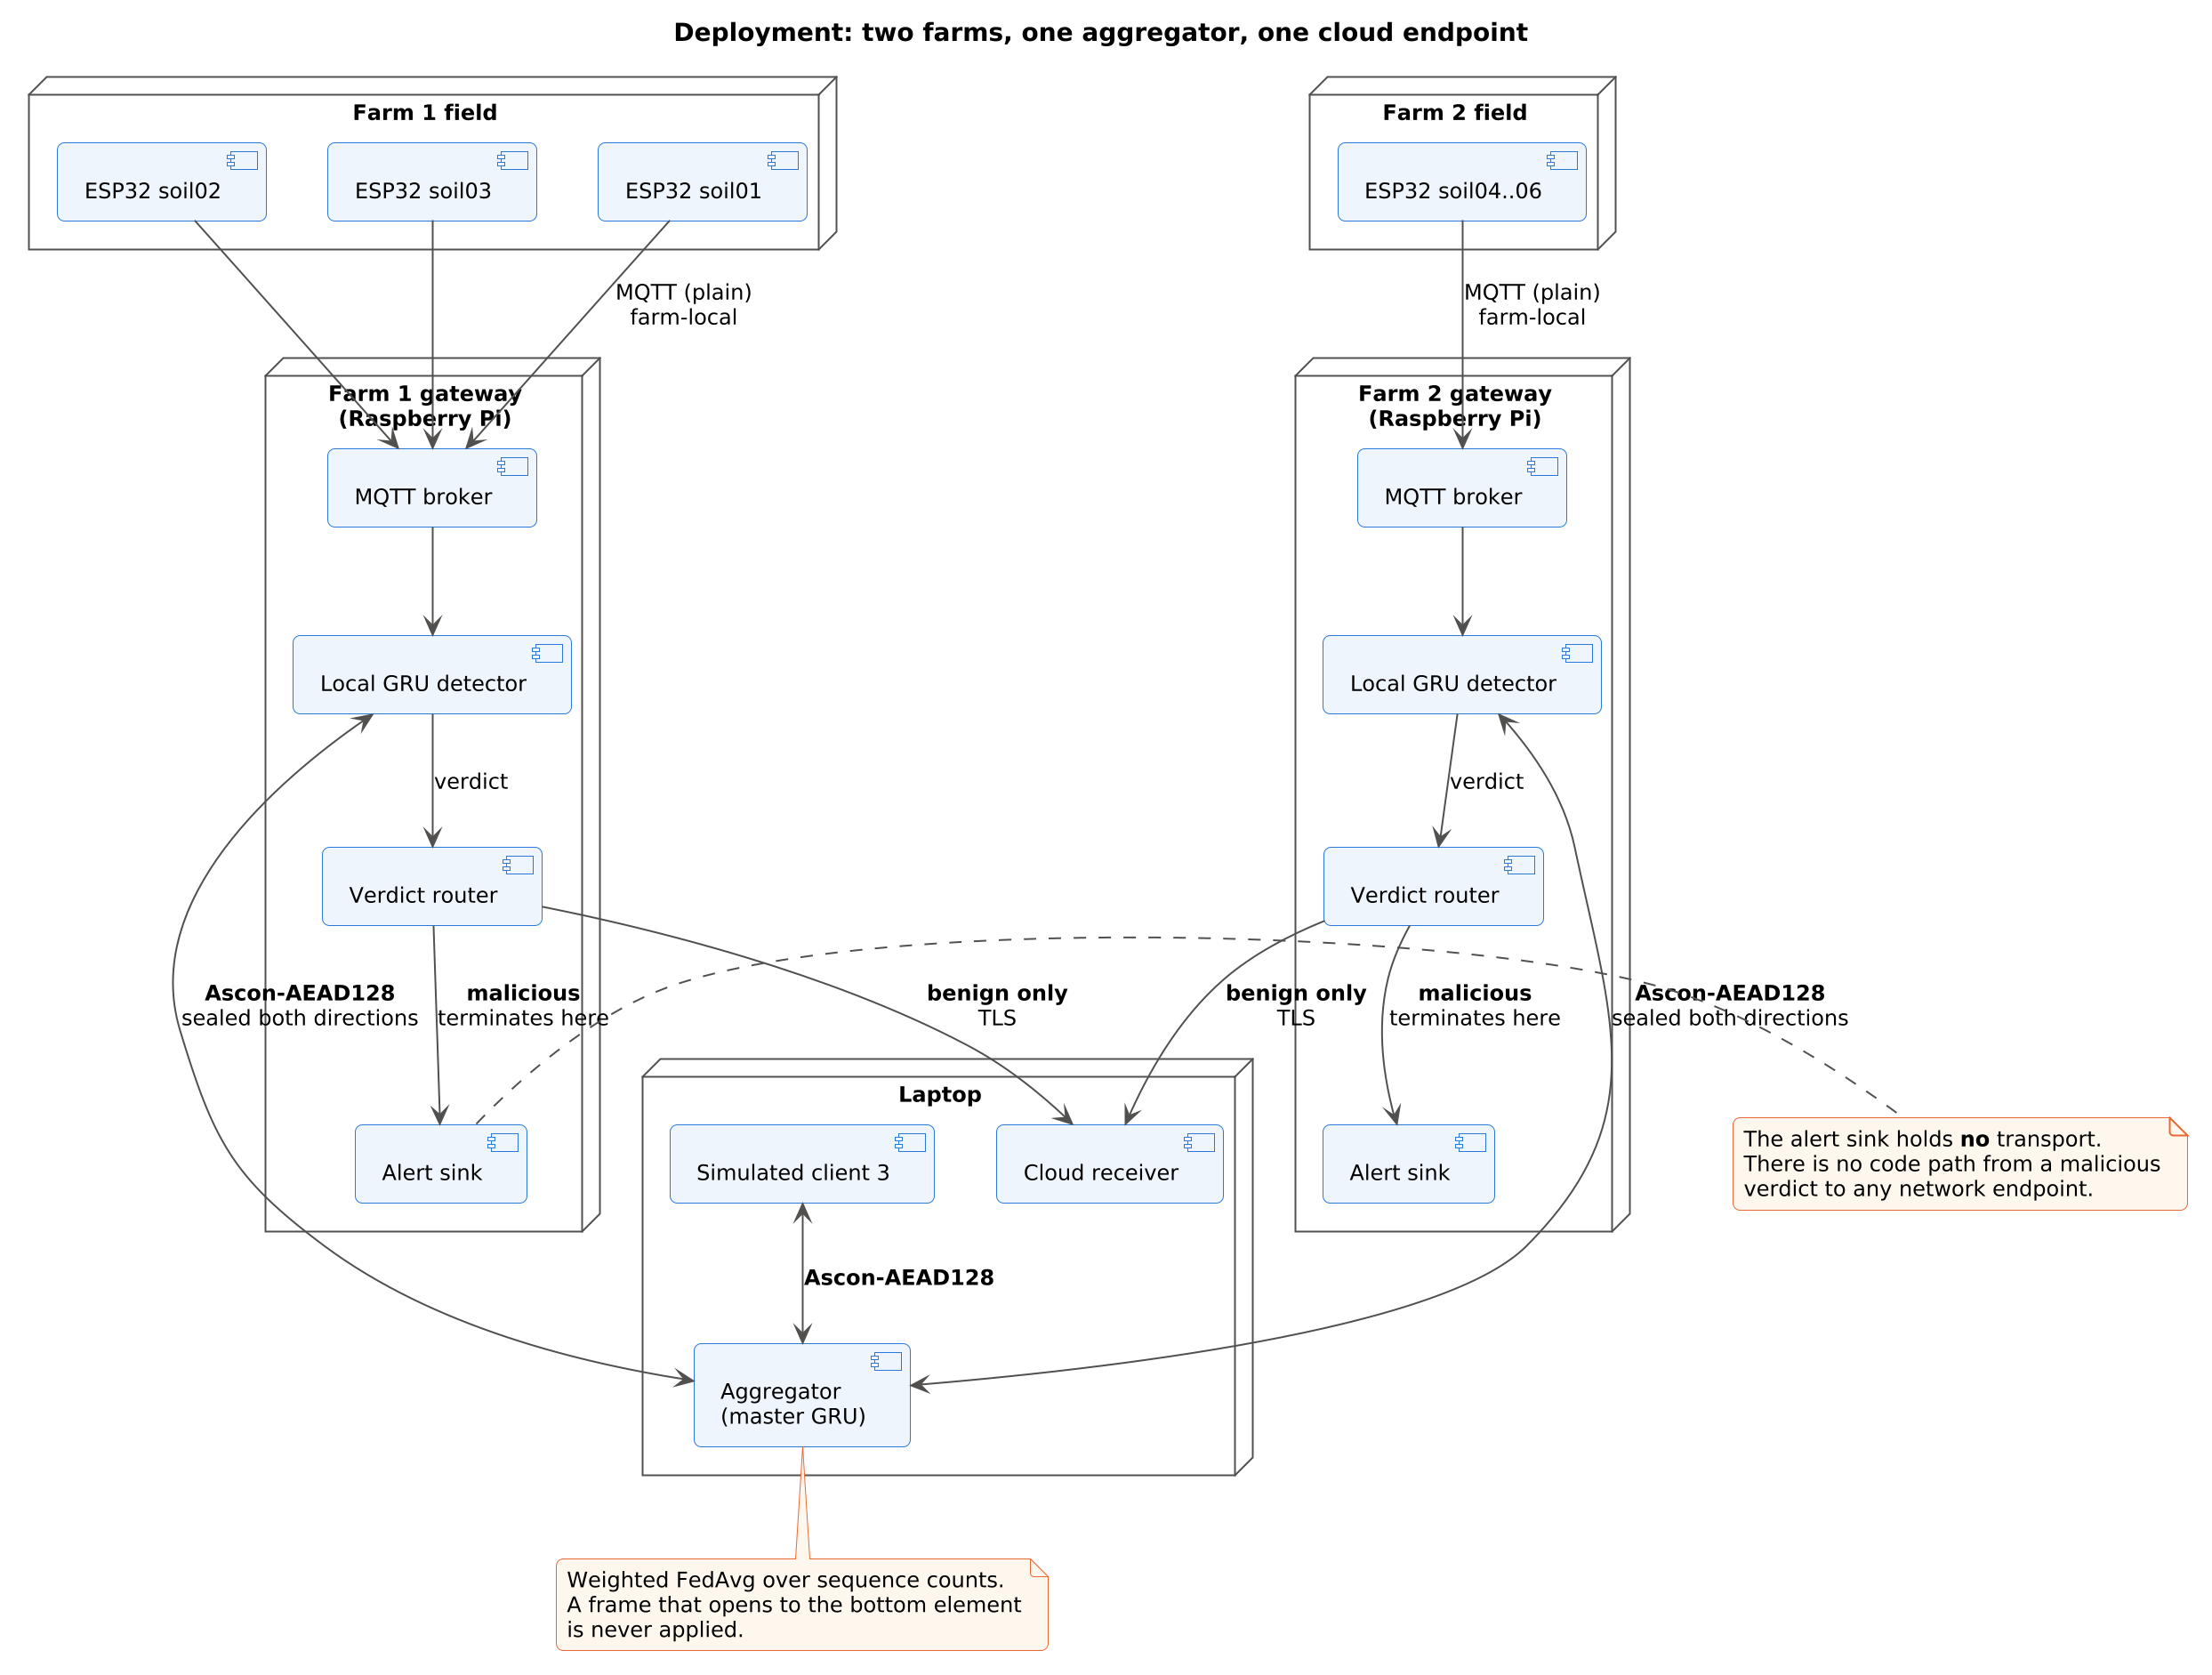
\includegraphics[width=0.96\textwidth]{01_deployment.png}
\caption{Deployment view, with the cryptographic protection named on each hop. Ascon-AEAD128
seals the parameter exchange in both directions; the gateway-to-cloud hop is TLS; the
malicious-verdict path has no network endpoint at all.}
\label{fig:arch}
\end{figure*}

\begin{figure}[t]\centering
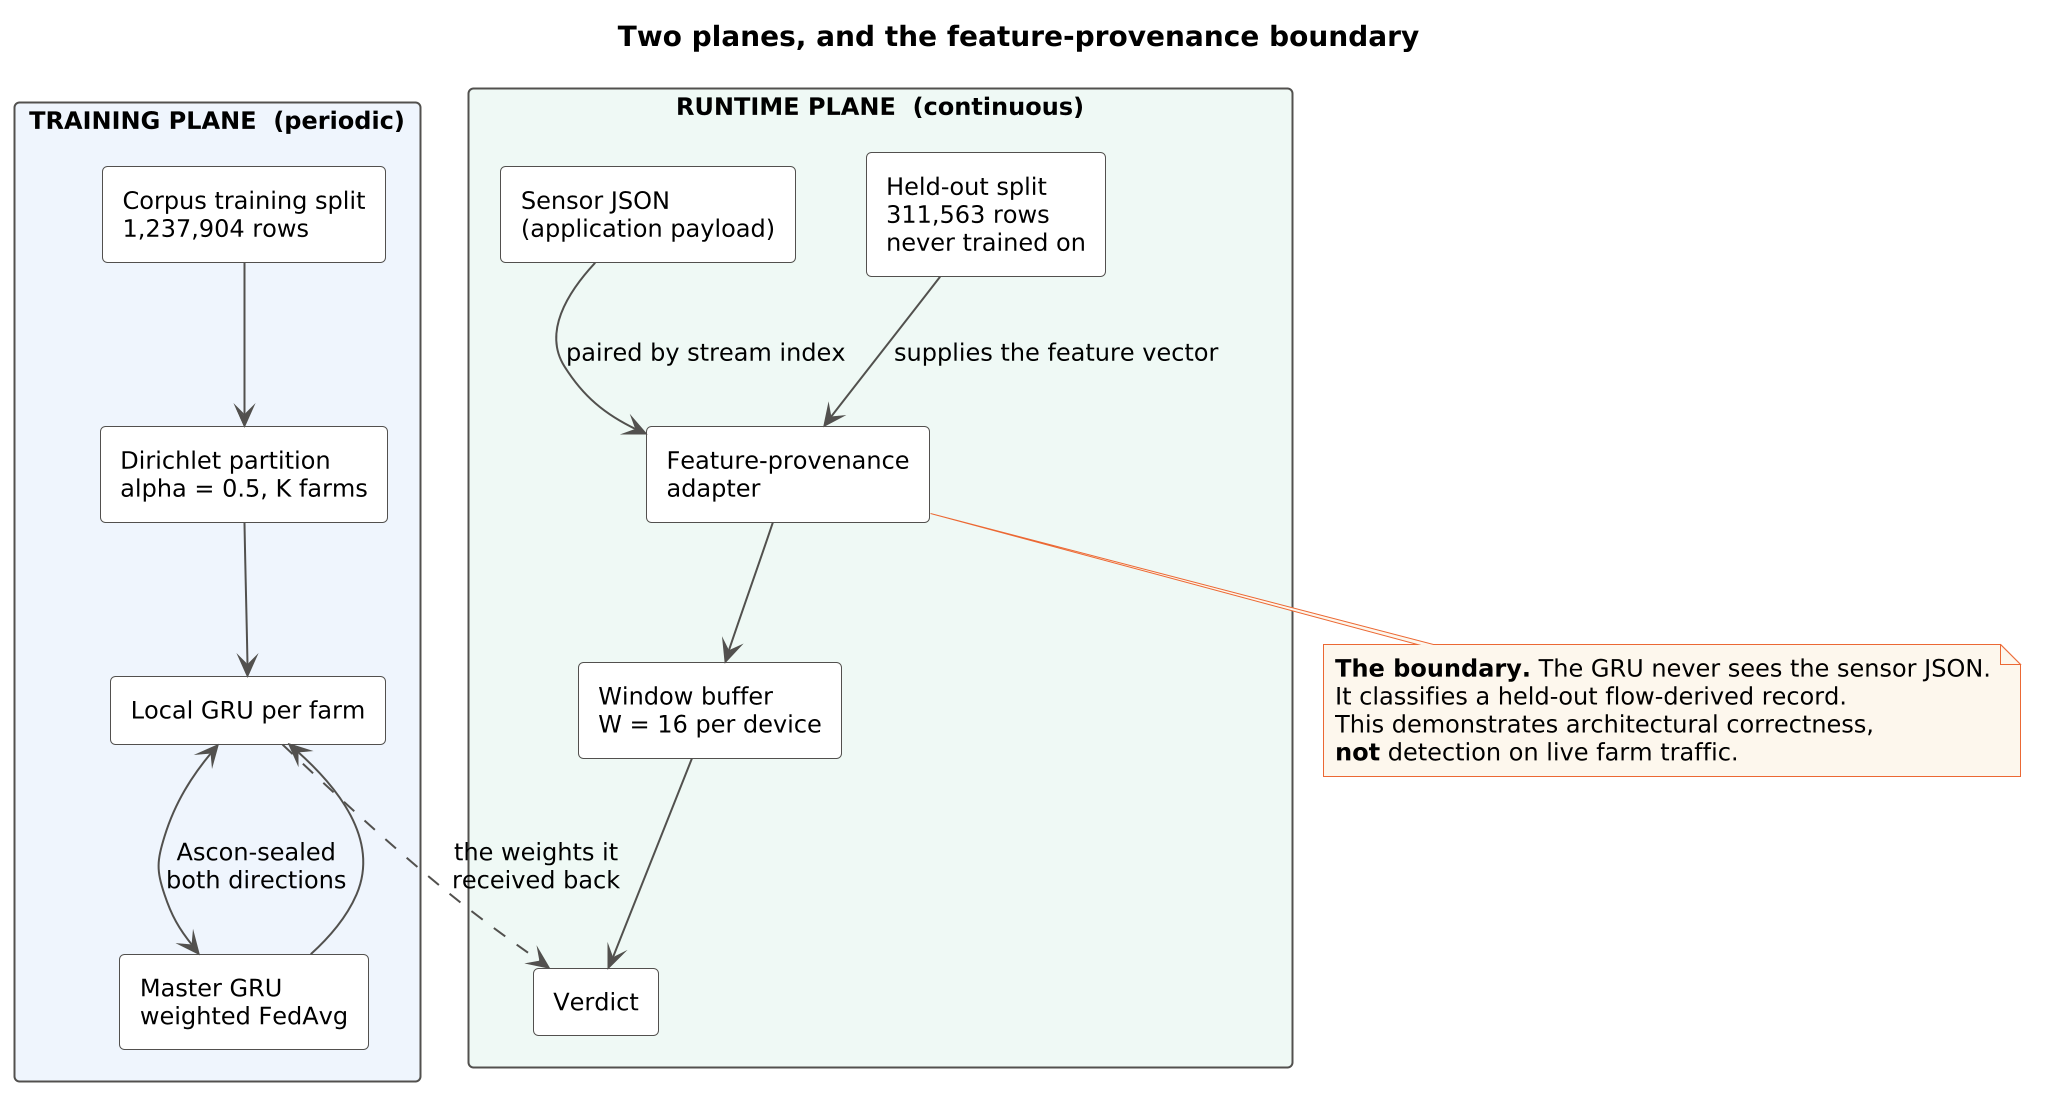
\includegraphics[width=\columnwidth]{04_two_planes.png}
\caption{The training plane, the runtime plane, and the feature-provenance boundary between
them. The detector never consumes the application payload.}
\label{fig:planes}
\end{figure}

%=======================================================================
\section{Methodology}

\subsection{Corpus, leakage control, and why one corpus}\label{sec:data}
\todo{write from docs/dataset-selection.md. Deduplicate before splitting; the ordering is the
control. Report the three corpora and the measurements that rejected two.}

\begin{algorithm}[t]
\caption{Leakage-controlled preparation}\label{alg:prep}
\begin{algorithmic}[1]
\Require raw capture parts $\mathcal{P}$, per-class cap $\kappa$, block size $b$, test fraction $\tau$
\State $D \gets \textsc{StratifiedCappedSubsample}(\mathcal{P}, \kappa)$
\State $D \gets \textsc{Deduplicate}(D)$ \Comment{before splitting, not after}
\State $\beta \gets \textsc{AssignBlocks}(D, b)$ \Comment{blocks never span a label}
\State $(\beta_{\text{tr}}, \beta_{\text{te}}) \gets \textsc{StratifiedBlockSplit}(\beta, \tau)$
\State \textbf{assert} $\textsc{Hashes}(D_{\text{tr}}) \cap \textsc{Hashes}(D_{\text{te}}) = \emptyset$
\State $S \gets \textsc{BuildWindows}(D_{\text{tr}})$ \Comment{within contiguous same-label runs}
\State \Return $(S, D_{\text{te}})$
\end{algorithmic}
\end{algorithm}

\subsection{Feature selection}
\todo{four stages, 39 $\rightarrow$ 16, with Fig.~3.}

\subsection{Temporal sequence construction}\label{sec:sequences}
Windows are built only over maximal runs of adjacent records sharing both label and source
capture. Rows are never shuffled before windowing; only complete sequences are shuffled at batch
formation. A window's label is that of its final record, $y_i = y_{i+W-1}$. The number of
sequences obtainable from runs of lengths $\{L_r\}$ at window $W$ is
\begin{equation}
N_{\text{seq}} = \sum_r \max(0,\; L_r - W + 1).
\label{eq:nseq}
\end{equation}

\subsection{Detection model}
\todo{GRU equations; LayerNorm not BatchNorm, because batch statistics do not aggregate across
federated clients.} The default configuration has $F=16$ input features, hidden width $H=96$ and
$C=8$ classes, giving
\begin{equation}
|\theta| = 3H(F + H + 1) + H(2 + C) + C = 33{,}800,
\label{eq:params}
\end{equation}
a figure asserted by a unit test so that a silent architecture change cannot pass review.

Class imbalance is handled by weighting the cross-entropy from \emph{training} counts only,
\begin{equation}
w_c = \frac{n}{C \, n_c},
\label{eq:classweights}
\end{equation}
with no synthetic oversampling, which would fabricate temporal structure the windowing rules
exist to preserve.

\subsection{Federated training}
Client $k$'s partition is drawn blockwise from a Dirichlet distribution,
\begin{equation}
(p_{1c},\dots,p_{Kc}) \sim \mathrm{Dir}(\alpha \mathbf{1}_K) \quad \text{per class } c,
\label{eq:dirichlet}
\end{equation}
with $\alpha$ an experimental variable rather than a fixed choice. Aggregation is weighted
FedAvg over \emph{sequence} counts, not raw row counts:
\begin{equation}
\theta^{(t+1)} = \sum_{k=1}^{K} \frac{n_k}{\sum_j n_j}\, \theta_k^{(t)},
\qquad n_k = |S_k|.
\label{eq:fedavg}
\end{equation}
Weighting by rows rather than sequences is a common and silent error, because windowing is not
length-preserving; Eq.~\eqref{eq:fedavg} is asserted by a test.

Standardisation is federated: each client contributes only count, mean and second-moment
statistics, combined by Chan's parallel formula,
\begin{align}
n_{AB} &= n_A + n_B, \qquad \delta = \mu_B - \mu_A, \label{eq:chan1}\\
\mu_{AB} &= \mu_A + \delta\,\frac{n_B}{n_{AB}}, \qquad
M_{2,AB} = M_{2,A} + M_{2,B} + \delta^2\frac{n_A n_B}{n_{AB}}. \label{eq:chan2}
\end{align}
No raw record leaves a client, and the federated scaler was measured equal to a pooled scaler to
within $5\times10^{-12}$ at every client count tested.

\begin{algorithm}[t]
\caption{One sealed federated round}\label{alg:round}
\begin{algorithmic}[1]
\Require global state $\theta^{(t)}$, clients $1..K$, keys $(k^{\uparrow}_i, k^{\downarrow}_i)$
\For{each client $i$ in parallel}
  \State $\theta_i \gets \textsc{LocalTrain}(\theta^{(t)}, S_i, E)$
  \State $a \gets \langle i,\, t,\, \textsf{up},\, v \rangle$;\quad $\nu \gets \textsc{Csprng}(128)$
  \State send $\textsc{Seal}(k^{\uparrow}_i, \nu, a, \textsc{Serialize}(\theta_i, n_i))$
\EndFor
\For{each received frame $f$ from client $i$}
  \State $m \gets \textsc{Open}(k^{\uparrow}_i, f)$
  \State \textbf{if} $m = \bot$ \textbf{then} reject and \textbf{continue} \Comment{never applied}
  \State $(\theta_i, n_i) \gets \textsc{Deserialize}(m)$
\EndFor
\State $\theta^{(t+1)} \gets \sum_i \frac{n_i}{\sum_j n_j}\theta_i$ \Comment{Eq.~\eqref{eq:fedavg}}
\For{each client $i$}
  \State $a' \gets \langle i,\, t,\, \textsf{down},\, v \rangle$;\quad $\nu' \gets \textsc{Csprng}(128)$
  \State send $\textsc{Seal}(k^{\downarrow}_i, \nu', a', \textsc{Serialize}(\theta^{(t+1)}))$
\EndFor
\end{algorithmic}
\end{algorithm}

\begin{figure}[t]\centering
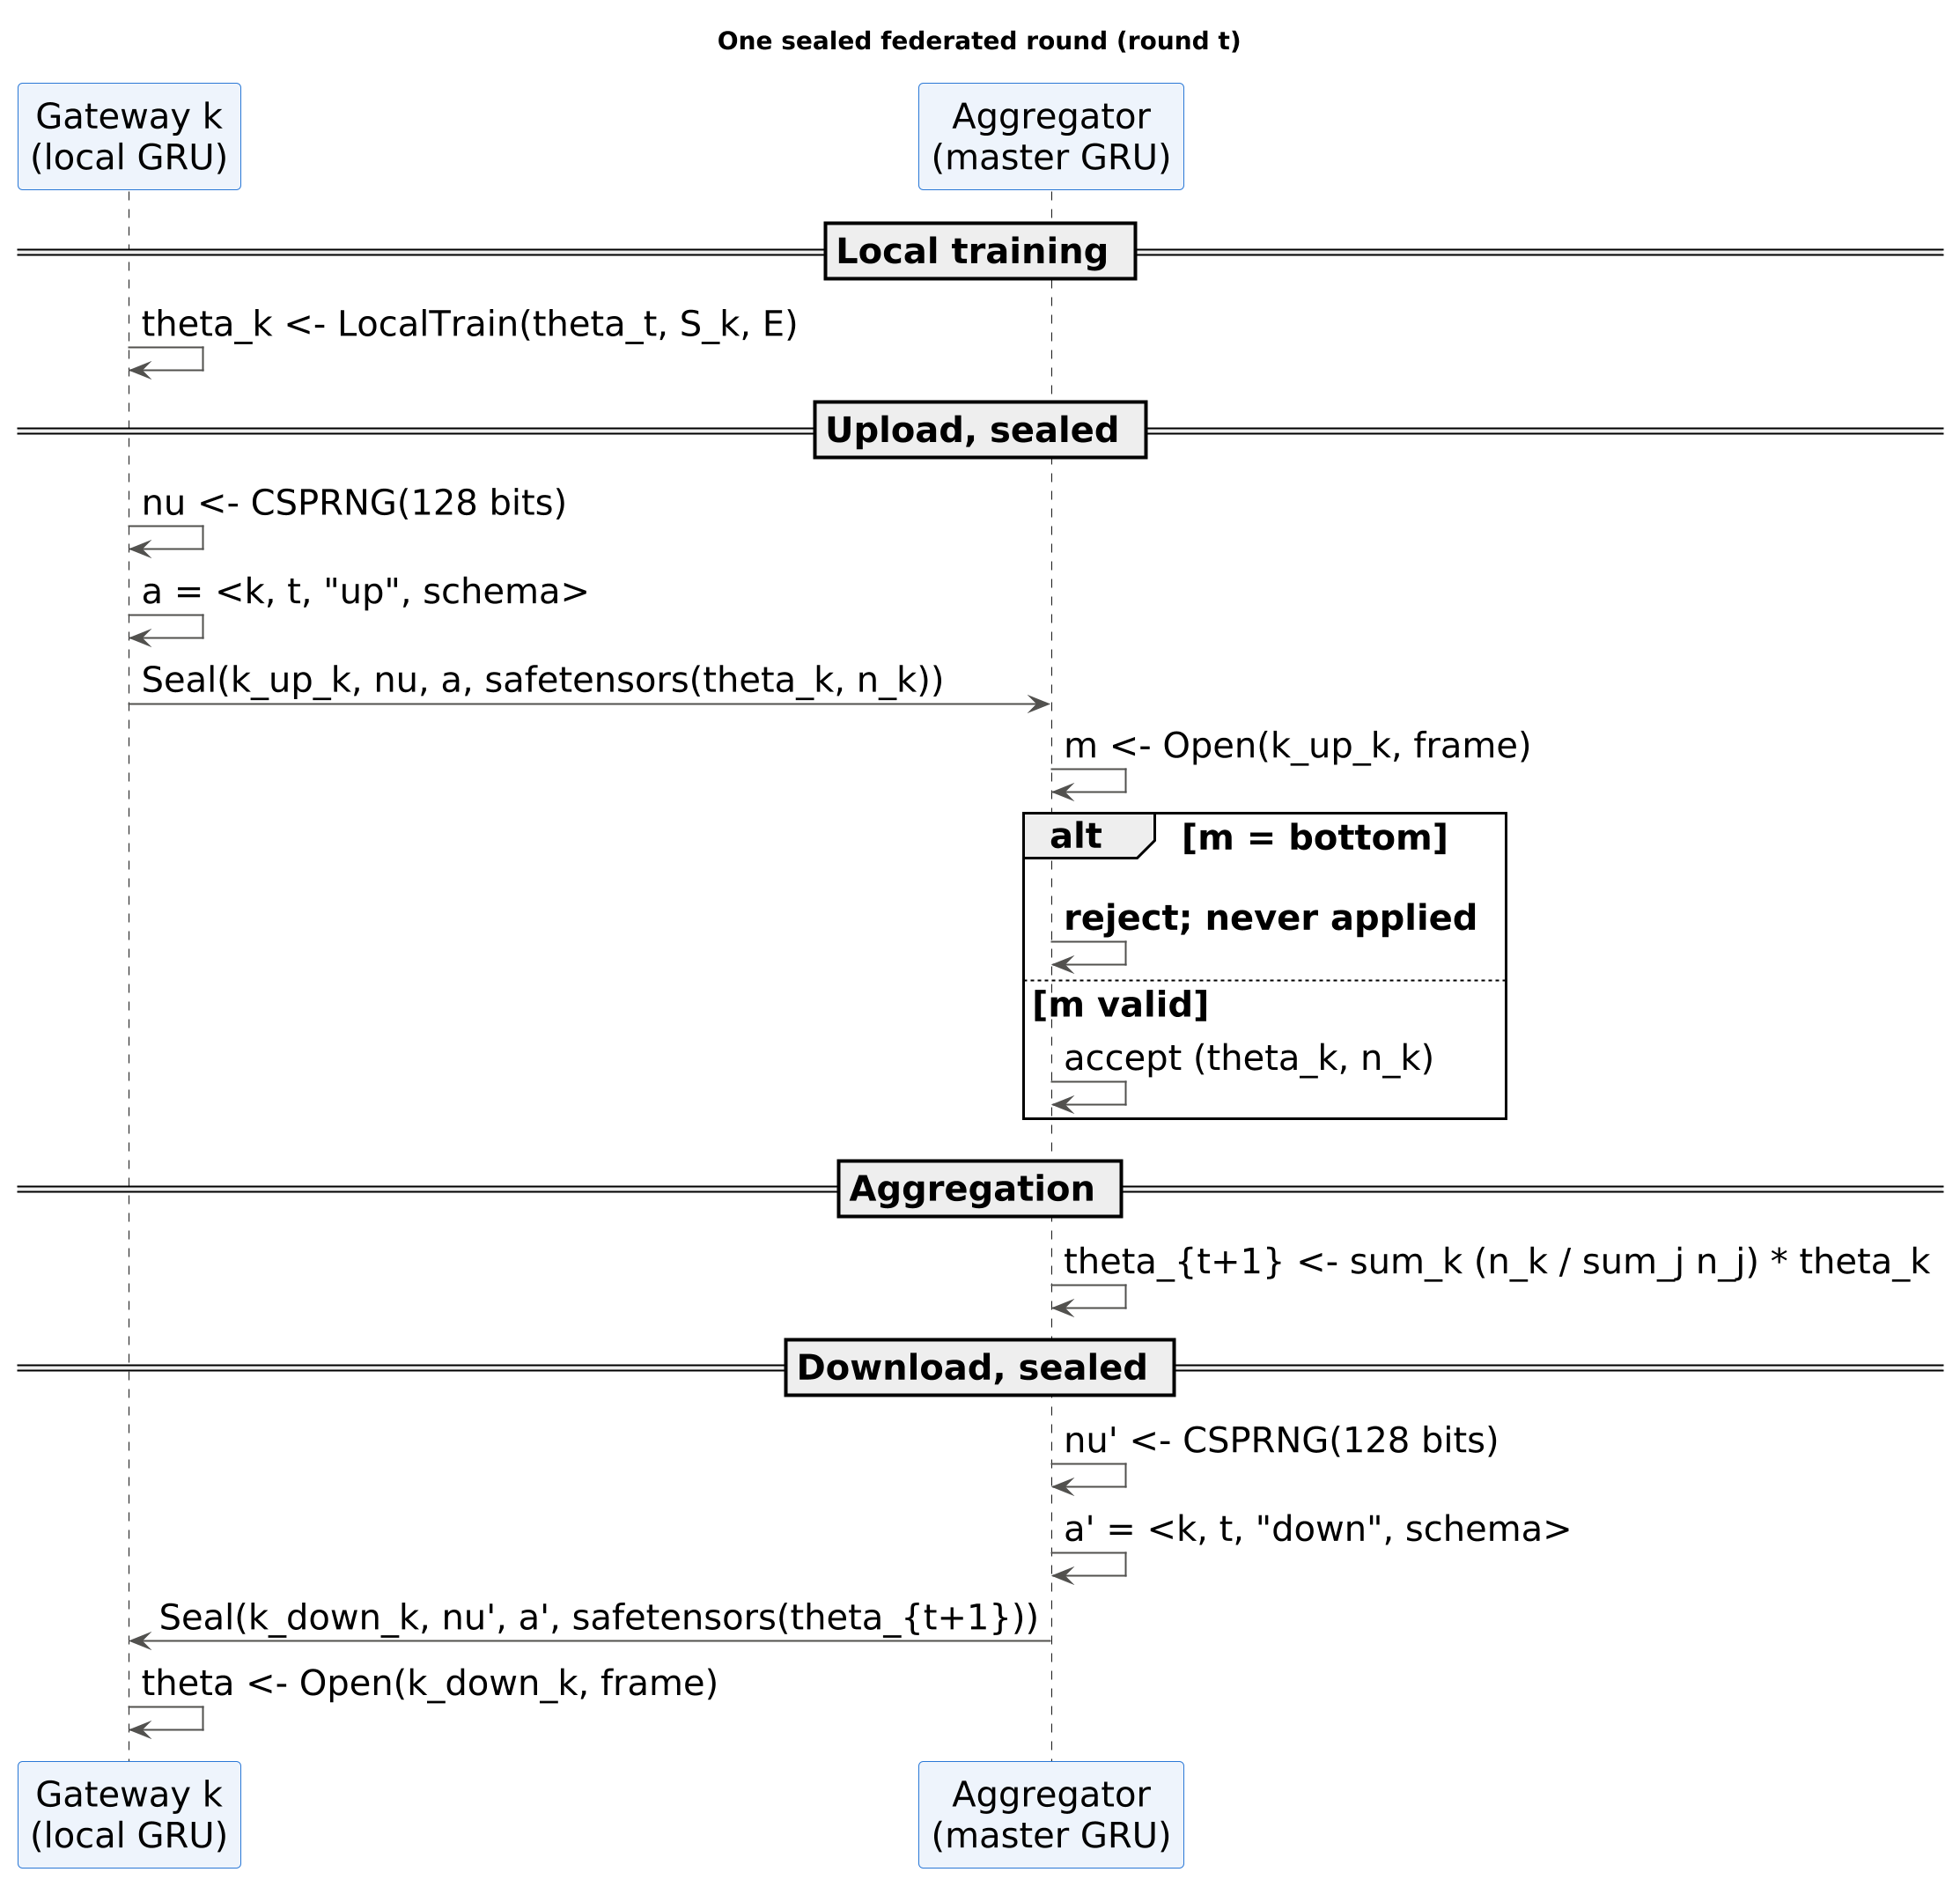
\includegraphics[width=\columnwidth]{02_sealed_round.png}
\caption{One sealed federated round. Keys are per client and per direction; the associated data
binds client, round, direction and schema version.}
\label{fig:round}
\end{figure}

\subsection{The sealed weight channel}\label{sec:channel}
Each frame carries associated data
\begin{equation}
a = \langle \texttt{client\_id},\; \texttt{round},\; \texttt{direction},\; \texttt{schema\_version} \rangle,
\label{eq:weightad}
\end{equation}
authenticated but not encrypted, so a frame cannot be replayed into a different round, reflected
into the opposite direction, attributed to a different client, or reinterpreted under a different
parameter layout. Keys are per client and per direction, nonces are drawn fresh from a CSPRNG for
every frame, and parameters are serialised with safetensors rather than pickle so that opening a
frame cannot execute code. Per-round traffic is
\begin{equation}
B = 2K\big(|\theta| s + h\big),
\label{eq:bytes}
\end{equation}
which predicts 811{,}200 bytes per round at $K=3$ against 815{,}136 measured, the
0.5\% excess being safetensors framing.

\begin{figure}[t]\centering
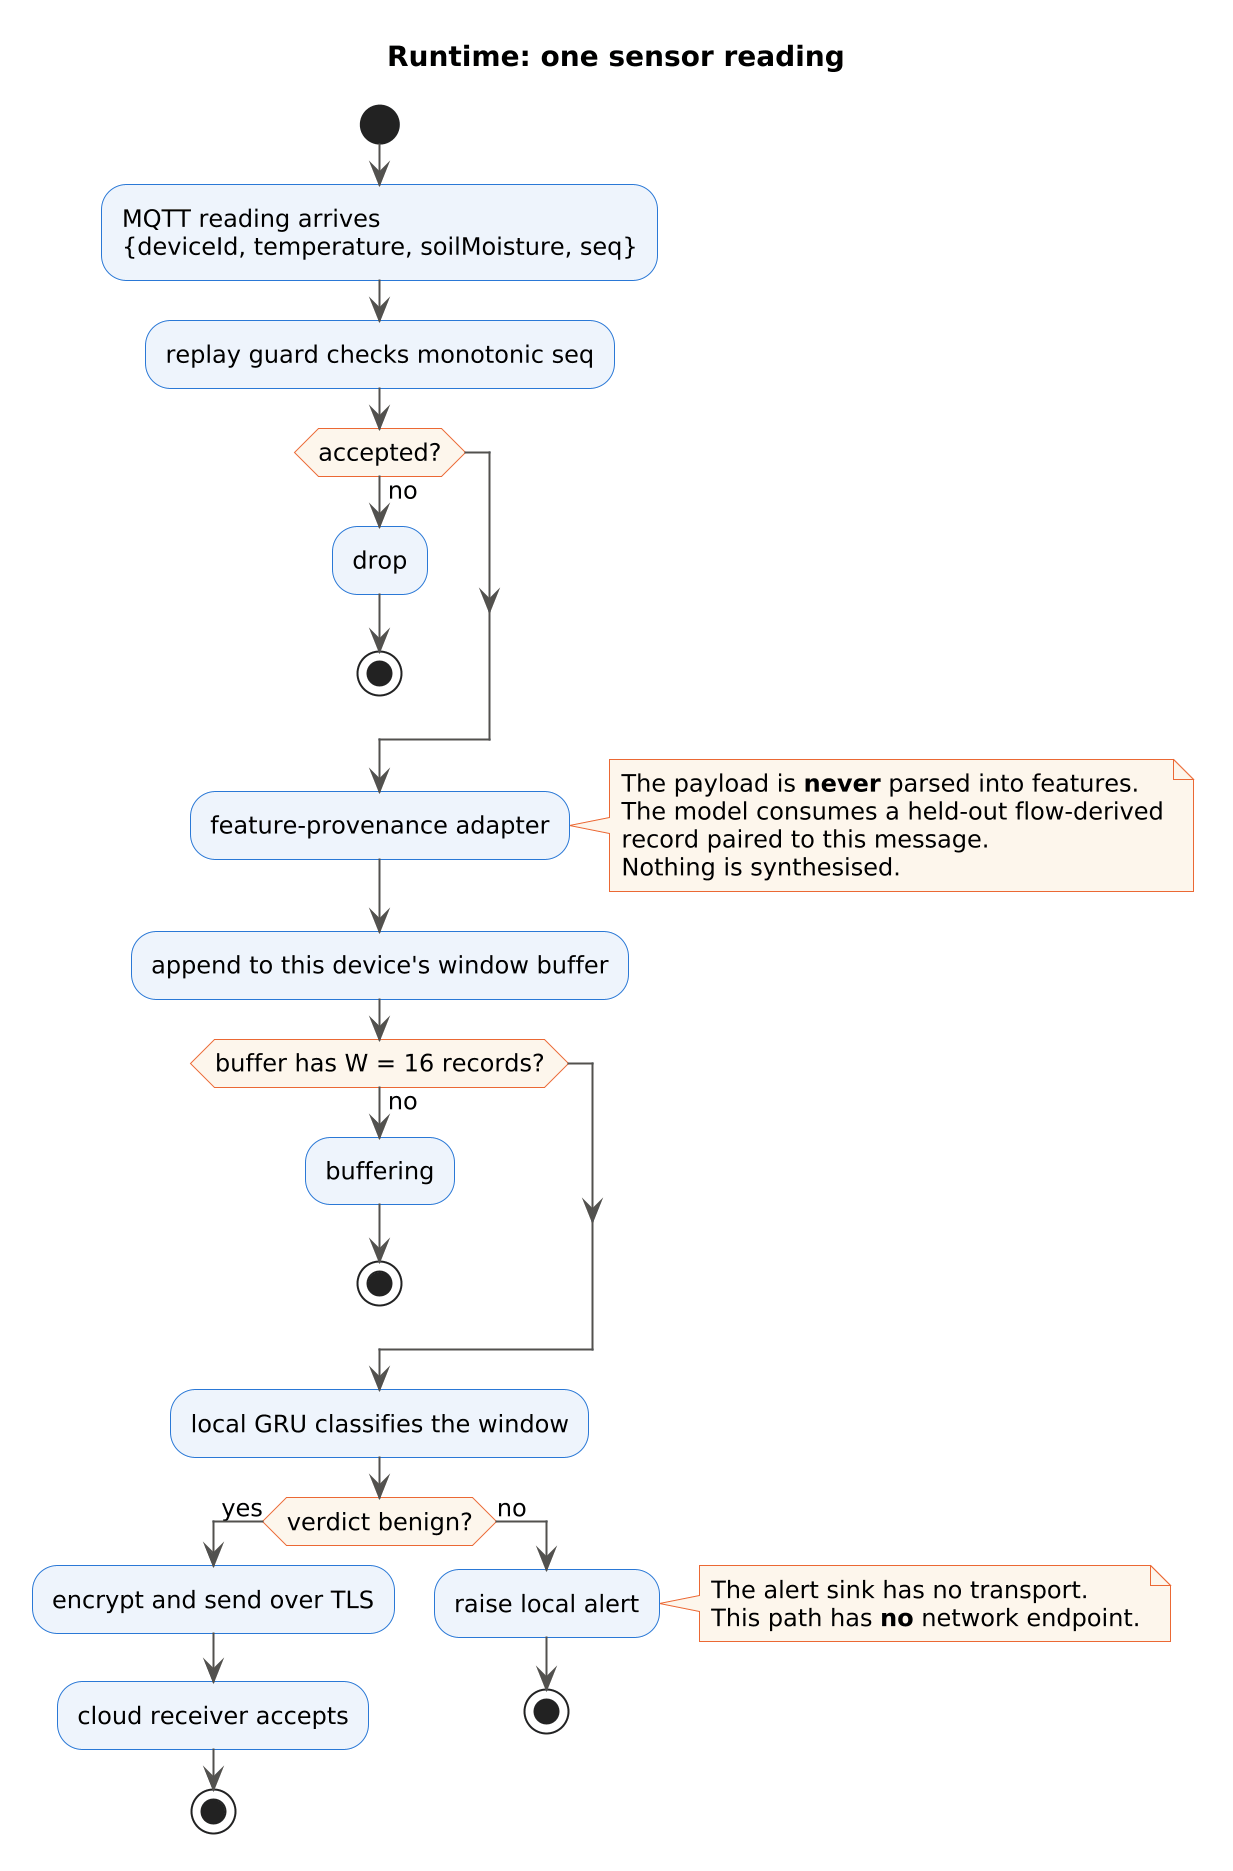
\includegraphics[width=\columnwidth]{03_verdict_routing.png}
\caption{The runtime path of a single reading. The malicious branch has no network endpoint.}
\label{fig:routing}
\end{figure}

\subsection{Verdict routing with disjoint paths}\label{sec:routing}
The verdict selects the path:
\begin{equation}
\text{path}(x) =
\begin{cases}
\text{TLS to cloud}, & \hat{y}(x) = \text{benign},\\
\text{local alert}, & \hat{y}(x) \neq \text{benign}.
\end{cases}
\label{eq:route}
\end{equation}
Disjointness is enforced in the object graph, not by a coding rule: the handler for malicious
verdicts is constructed with no arguments at all and therefore holds no transport it could reach
the network with. Breaking the property requires changing a constructor signature, which three
tests reject.

\subsection{Runtime feature provenance}\label{sec:provenance}
\todo{state the boundary: the model consumes held-out flow-derived records paired to each
arriving message; the application payload is never parsed into features; the scenario control
selects which held-out pool is drawn from and synthesises nothing. Say plainly what this
demonstrates (architectural correctness) and what it does not (detection on live farm traffic).}

%=======================================================================
\section{Experimental Setup}
\todo{corpus splits, budgets, seeds, hardware, and the statement that every reported figure is
read from a committed run manifest rather than transcribed.}

%=======================================================================
\section{Results}

\begin{figure}[t]\centering
\includegraphics[width=\columnwidth]{baselines.pdf}
\caption{Centralised baselines at an identical budget and split. Recurrence is worth $+0.2322$
macro-F1 against the otherwise-matched multilayer perceptron.}
\label{fig:baselines}
\end{figure}

\subsection{Centralised baselines and the value of recurrence}
\todo{table: random forest 0.6855, MLP 0.6070, GRU 0.8297 $\pm$ 0.0013 at $W\!=\!16$, three
seeds, identical split and budget. Recurrence is worth $+0.2322$, fifty-one times the seed
standard deviation.}

\begin{figure}[t]\centering
\includegraphics[width=\columnwidth]{federation_bracket.pdf}
\caption{The three-way comparison. The federated model sits inside the bracket its two baselines
define, recovering 82.4\% of the gap.}
\label{fig:bracket}
\end{figure}

\begin{figure}[t]\centering
\includegraphics[width=\columnwidth]{per_client_gain.pdf}
\caption{What each farm gains by federating rather than training alone, on both corpora. Every
bar is positive on every seed.}
\label{fig:gain}
\end{figure}

\subsection{Federated performance and per-client gain}\label{sec:fedresults}
\todo{bracket table and Fig.~6--7. Federated $0.8308 \pm 0.0150$ between local-only
$0.7205 \pm 0.0750$ and centralised $0.8543 \pm 0.0040$, recovering 82.4\%. Per-client gains all
positive. Read FPR $0.2975 \pm 0.0512$ first.}

\subsection{Client-count scalability}\label{sec:ksweep}
Table~\ref{tab:ksweep} reports 21 configurations, three seeds each, at the Phase-4 budget.

\begin{table}[t]
\caption{Client-count sweep. Three seeds per row. ``Rarest'' is the mean per-class F1 of the
weakest class at that client count.}
\label{tab:ksweep}
\centering\small
\begin{tabular}{@{}rccccr@{}}
\toprule
$K$ & macro-F1 & FPR & Rarest & Seq./client & MB/round\\
\midrule
3  & $\mathbf{0.8367 \pm 0.0107}$ & $0.2988$ & $\mathbf{0.642}$ & 399{,}424 & 0.82\\
5  & $0.7835 \pm 0.0340$ & $0.3366$ & $0.564$ & 238{,}361 & 1.36\\
10 & $0.7974 \pm 0.0195$ & $0.2144$ & $0.557$ & 118{,}012 & 2.72\\
20 & $0.7866 \pm 0.0260$ & $0.1765$ & $0.531$ & 58{,}618  & 5.43\\
30 & $0.7863 \pm 0.0001$ & $0.3149$ & $0.513$ & 38{,}979  & 8.15\\
40 & $0.7778 \pm 0.0091$ & $0.3184$ & $0.466$ & 29{,}215  & 10.87\\
50 & $0.7577 \pm 0.0134$ & $\mathbf{0.3882}$ & $\mathbf{0.386}$ & 23{,}355 & 13.59\\
\bottomrule
\end{tabular}
\end{table}

The curve has three regimes. From $K=3$ to $K=5$ aggregate macro-F1 drops $0.053$ as each
client's partition falls below the sequence cap, so the cap stops binding. From $K=5$ to $K=30$
it is flat: a sixfold increase in client count costs $0.004$, and at $K=30$ the spread across
seeds is $\pm 0.0001$. A second descent then begins, $0.7863 \rightarrow 0.7778 \rightarrow
0.7577$, which is not an artefact of the aggregate. The onset coincides with the pigeonhole
bound on client count implied by the rarest class,
\begin{equation}
K^{\dagger} = \min_c |\beta_c| = 42,
\label{eq:pigeonhole}
\end{equation}
past which some client must hold zero blocks of class $c$ regardless of the draw.

\textbf{The aggregate conceals the finding.} The weakest class falls monotonically at every step,
$0.642 \rightarrow 0.564 \rightarrow 0.557 \rightarrow 0.531 \rightarrow 0.513 \rightarrow 0.466
\rightarrow 0.386$: a $-0.256$ absolute and 40\% relative collapse, while macro-F1 moves only
$-0.079$ because the easiest class holds $0.998$ throughout. Reporting macro-F1 alone would have
hidden it, and the false-positive rate---worst at $K=50$---tracks the collapse more faithfully
than macro-F1 does. No client was ever empty, at any $K$ including 50, so the mechanism is
dilution of the rare class rather than its absence.

\begin{figure}[t]\centering
\includegraphics[width=\columnwidth]{ksweep_f1.pdf}
\caption{Aggregate macro-F1 degrades gently with client count while the weakest class collapses.
Both series are F1 on a single axis, which is the point: the aggregate conceals the rare-class
fall. The second descent begins at the pigeonhole bound of Eq.~\eqref{eq:pigeonhole}.}
\label{fig:ksweep}
\end{figure}

\begin{figure}[t]\centering
\includegraphics[width=\columnwidth]{communication.pdf}
\caption{Per-round traffic against client count. Plotted separately from
Fig.~\ref{fig:ksweep} because bytes and F1 do not share a scale.}
\label{fig:comm}
\end{figure}

\begin{figure}[t]\centering
\includegraphics[width=\columnwidth]{convergence.pdf}
\caption{Per-round macro-F1 at three client counts, seed 0. Higher client counts converge no more
slowly; they converge lower.}
\label{fig:convergence}
\end{figure}

\subsection{Cryptographic and communication overhead}
\todo{table: per-round bytes measured against Eq.~\eqref{eq:bytes}; seal/open latency; and the
observation that communication grows linearly to 13.59\,MB per round at $K=50$,
so the benefit degrades before the communication break-even is reached.}

\begin{figure}[t]\centering
\includegraphics[width=\columnwidth]{feature_overlap.pdf}
\caption{Cross-corpus overlap of each selected feature's 1st--99th percentile range. Three
features share a column name while denoting different quantities; \texttt{IAT} medians differ by
a factor of $2.4\times10^{11}$.}
\label{fig:overlap}
\end{figure}

\subsection{Dataset selection as a result}\label{sec:semantics}
\todo{write from docs/dataset-selection.md and docs/generalisation-plan.md: the three corpora,
the two rejections and their measurements, the $7.33\times$ extractor window-size difference, and
the three columns whose ranges are disjoint---including \texttt{Variance} spanning $0..1$ in one
corpus and $0..1.13\times10^{8}$ in the other.}

\subsection{Zero-shot cross-corpus transfer: a replication}
\todo{report our figures and frame them as a replication of
\cite{layeghy2022generalisability}---56.28\% average decay across four corpora sharing a single
standardised 43-feature schema---and of \cite{dataset_centric_fl_ids}'s up-to-30-point loss. Note
that schema standardisation does not rescue transfer, so our semantics defect is not the cause.}

%=======================================================================
\section{Software-in-the-Loop Validation}\label{sec:sil}
We validated the complete topology before any hardware existed. By
\emph{software-in-the-loop} we mean precisely: the production node software, unmodified,
executing as separate operating-system processes on a real network at the target CPU
architecture, with sensor inputs supplied by a contract-equivalent simulator. Ten containers
stood in for two farm gateways, their two brokers, six sensor nodes, the aggregator, the cloud
receiver and a one-shot key provisioning step. \emph{Container timings are not gateway timings};
every manifest records the platform so no timing figure can be mistaken for a hardware
measurement. On-device validation (hardware-in-the-loop) is future work.

\begin{table}[t]
\caption{Software-in-the-loop run, 20 federated rounds then continuous classification.}
\label{tab:sil}
\centering\small
\begin{tabular}{@{}lrrr@{}}
\toprule
 & Gateway 1 & Gateway 2 & Total\\
\midrule
Sealed frames (both directions) & \multicolumn{2}{c}{120} & \textbf{0 rejected}\\
Bytes per client per round      & \multicolumn{3}{c}{271{,}883}\\
\midrule
Readings received        & 6{,}626 & 6{,}627 & 13{,}253\\
Benign $\rightarrow$ cloud & 5{,}421 & 3{,}503 & 8{,}924\\
\quad failed sends         & 0 & 0 & \textbf{0}\\
Malicious $\rightarrow$ local alert & 1{,}160 & 3{,}079 & \textbf{4{,}239}\\
\textbf{Malicious reaching cloud}   & \textbf{0} & \textbf{0} & \textbf{0}\\
\bottomrule
\end{tabular}
\end{table}

The receiver's own independent count was 8{,}924 accepted and zero rejected, matching the sum of
what the two gateways sent, so the disjointness result is not a self-report.

\subsection{A safety property can pass vacuously}\label{sec:vacuous}
An earlier run of this same configuration reported the disjointness property satisfied, on
\emph{one} malicious reading: the sensor simulators began publishing before the gateways had
finished federating, and the broker's quality-of-service level discards messages published before
a subscription exists. The assertion held and established nothing. A system leaking one malicious
reading in ten would have passed that test with probability $0.9$; at 4{,}239 readings the same
system passes with probability $1.1\times10^{-194}$.

We therefore state the general form as a gap: \emph{a safety property reported as satisfied
carries no information unless the number of opportunities to violate it is reported alongside.}
We report both throughout.

%=======================================================================
\section{Limitations and Threats to Validity}\label{sec:limitations}
\todo{write from docs/paper-claims-inventory.md Section B, in our own voice and before a reviewer
raises them: the feature-provenance boundary means detection on live farm traffic is not
demonstrated; cross-corpus transfer was measured and failed; Ascon protects the parameter channel
and not the telemetry; no on-device results yet, so no timing claim; $K=3$ is a budget constraint;
leave-one-device-out could not be run because the corpus carries no device attribution; and
gradient inversion, poisoning, differential privacy and secure aggregation are all out of scope.}

%=======================================================================
\section{Conclusion}
\todo{write last.}

%=======================================================================
\bibliographystyle{IEEEtran}
\bibliography{references}

\end{document}
